% =====================================================================
%  CPE 333 Operating Systems 1/2569 - Problem Session 6
%  Virtual Memory
%  ---------------------------------------------------------------
%  คอมไพล์ด้วย XeLaTeX
% =====================================================================
\documentclass[a4paper,11pt]{article}

% ------------------------- Layout -------------------------
\usepackage[margin=2.2cm,top=2.2cm,bottom=2.2cm]{geometry}
\usepackage{fancyhdr}
\setlength{\headheight}{14pt}
\usepackage{parskip}
\setlength{\parskip}{4pt}
\usepackage{enumitem}
\setlist{topsep=3pt,itemsep=2pt,parsep=0pt}
\usepackage{booktabs}
\usepackage{graphicx}
\usepackage{float}
\usepackage{caption}
\captionsetup{font=small,skip=3pt}
\usepackage{xcolor}
\usepackage{listings}
\usepackage[hidelinks]{hyperref}

% ------------------------- ฟอนต์ภาษาไทย -------------------------
\usepackage{fontspec}
\usepackage{xltxtra}

\setmainfont{TH Sarabun New}[Scale=1.45]
\setmonofont{Consolas}[Scale=0.78]

% การตัดคำภาษาไทย
\XeTeXlinebreaklocale "th"
\XeTeXlinebreakskip = 0pt plus 0.3pt
\emergencystretch=3em

% ------------------------- สไตล์โค้ด -------------------------
\definecolor{codebg}{RGB}{248,248,248}
\definecolor{codeframe}{RGB}{221,221,221}
\definecolor{kw}{RGB}{0,86,179}
\definecolor{cmt}{RGB}{106,153,85}
\definecolor{str}{RGB}{163,21,21}
\definecolor{numgray}{RGB}{150,150,150}

\lstdefinestyle{cstyle}{
  language=C,
  backgroundcolor=\color{codebg},
  frame=single,
  rulecolor=\color{codeframe},
  basicstyle=\ttfamily\scriptsize,
  keywordstyle=\color{kw}\bfseries,
  commentstyle=\color{cmt}\itshape,
  stringstyle=\color{str},
  numbers=left,
  numberstyle=\tiny\color{numgray},
  numbersep=6pt,
  showstringspaces=false,
  breaklines=true,
  breakatwhitespace=true,
  tabsize=4,
  captionpos=b,
  aboveskip=6pt,
  belowskip=2pt,
  xleftmargin=12pt,
  framexleftmargin=12pt,
  morekeywords={free,vmstat,swapon,swapoff,mkswap,fallocate,sysctl,swappiness,resmon,dd,systemctl},
}

\lstdefinestyle{terminal}{
  language={},
  keywordstyle=\relax,
  commentstyle=\relax,
  stringstyle=\relax,
  backgroundcolor=\color{codebg},
  frame=single,
  rulecolor=\color{codeframe},
  basicstyle=\ttfamily\scriptsize,
  numbers=none,
  breaklines=true,
  showstringspaces=false,
  captionpos=b,
  aboveskip=6pt,
  belowskip=2pt,
  xleftmargin=4pt,
}

\lstset{style=cstyle}
\renewcommand{\lstlistingname}{Code}
\newcommand{\code}[1]{\texttt{#1}}

% ------------------------- Header / Footer -------------------------
\pagestyle{fancy}
\fancyhf{}
\lhead{\small CPE 333 Operating Systems 1/2569}
\rhead{\small Problem Session 6}
\cfoot{\thepage}
\renewcommand{\headrulewidth}{0.4pt}


% =====================================================================
\begin{document}

% ------------------------- หน้าปก -------------------------
\begin{titlepage}
\centering
\vspace*{0.3cm}

\includegraphics[width=3.2cm]{KMUTT_CI_Primary_Logo-Full-1200x1200.png}\\[0.8cm]
{\Large\bfseries รายงานปฏิบัติการ}\\[0.4cm]
{\Large\bfseries PS06: Virtual Memory}\\[0.4cm]
\vfill
{\large\bfseries เสนอ}\\[0.3cm]
{\large อาจารย์ ราชวิชช์ สโรชวิกสิต}\\[1.2cm]
{\large\bfseries จัดทำโดย}\\[0.4cm]
\renewcommand{\arraystretch}{1.35}
\begin{tabular}{l@{\hspace{1.5cm}}l}
นายภูมิพัฒน์ อภิวาทธนะพงศ์ & 67070501035 \\
นายวิรชัช ทองอุทัยศรี & 67070501041 \\
นายเจษฎา เกียรติกมลวงศ์ & 67070501080 \\
\end{tabular}
\renewcommand{\arraystretch}{1.0}
\vfill
{\large รายงานนี้เป็นส่วนหนึ่งของวิชา CPE 333 Operating Systems}\\[0.2cm]
{\large ภาควิชาวิศวกรรมคอมพิวเตอร์ คณะวิศวกรรมศาสตร์}\\[0.2cm]
{\large ภาคการศึกษาที่ 1 ปีการศึกษา 2569}\\[0.2cm]
{\large มหาวิทยาลัยเทคโนโลยีพระจอมเกล้าธนบุรี}
\end{titlepage}

% หน้าปกและสารบัญไม่นับเลขหน้า เนื้อหาจริงเริ่มนับที่หน้า 1
\thispagestyle{empty}
\tableofcontents
\newpage
\setcounter{page}{1}

% =====================================================================
\section*{สภาพแวดล้อมที่ใช้ในการทดลอง}
\addcontentsline{toc}{section}{สภาพแวดล้อมที่ใช้ในการทดลอง}
% =====================================================================

ปฏิบัติการนี้แบ่งการทดลองออกเป็นสองฝั่ง คือฝั่ง Linux (ข้อ 1 และข้อ 2) และฝั่ง MS Windows (ข้อ 3) โดยทั้งสองฝั่งทำงานอยู่บนเครื่องคอมพิวเตอร์เดียวกัน รายละเอียดของสภาพแวดล้อมเป็นดังนี้

\begin{table}[H]
\centering\small
\caption{ข้อมูลสภาพแวดล้อมของระบบที่ใช้ในการทดลอง}
\begin{tabular}{@{}p{3.9cm}p{12.2cm}@{}}
\toprule
\textbf{รายการ} & \textbf{รายละเอียด} \\
\midrule
ระบบปฏิบัติการฝั่ง Windows & Windows 11 Home Single Language (build 26200) \\
ระบบปฏิบัติการฝั่ง Linux & Ubuntu 24.04.1 LTS ทำงานบน WSL2 \\
Kernel ของ Linux & \code{6.6.87.2-microsoft-standard-WSL2} (x86-64) \\
หน่วยความจำหลักที่ Linux เห็น & 15 GiB (WSL2 แบ่งมาจาก RAM ของเครื่อง) \\
Swap เดิมของระบบ Linux & 4 GiB เป็น partition \code{/dev/sdc} ที่ WSL2 สร้างให้อัตโนมัติ \\
init ของ Linux & \code{systemd} (เปิดผ่าน \code{systemd=true} ใน \code{/etc/wsl.conf}) \\
เครื่องมือ monitoring & \code{procps-ng 4.0.4} ซึ่งเป็น package ที่ให้ทั้ง \code{free} และ \code{vmstat} \\
เครื่องมือฝั่ง Windows & Resource Monitor (\code{resmon.exe}) ที่มากับระบบปฏิบัติการ \\
\bottomrule
\end{tabular}
\end{table}

\textbf{หมายเหตุเรื่องหลักฐาน:} เนื่องจากใบงานกำหนดให้แสดงภาพหน้าจอของผลการรันคำสั่ง (ข้อ 1.2 ระบุ \textit{with screenshots} และข้อ 2 ระบุ \textit{Please capture the output image from running the command}) รายงานฉบับนี้จึงใช้ภาพหน้าจอจริงเป็นหลักฐานของทุกขั้นตอน ตัวเลขทุกตัวที่อ้างถึงในคำอธิบายและย่อหน้าสรุปอ่านมาจากภาพที่แสดงไว้ในรายงานโดยตรง ภาพทั้งหมดเก็บไว้ที่ \code{PS06/result/screenshots/} และลำดับคำสั่งที่ใช้ถ่ายภาพอยู่ใน \code{PS06/docs/COMMANDS.md}

% =====================================================================
\section{ข้อ 1: ทำความเข้าใจแนวคิดของ Virtual Memory}
% =====================================================================

\subsection{หลักการพื้นฐานที่ระบบปฏิบัติการสมัยใหม่ใช้ร่วมกัน}

Virtual Memory คือกลไกที่ระบบปฏิบัติการสร้าง address space เสมือนขึ้นมาให้แต่ละ process โดย address ที่ program มองเห็น (virtual address) ไม่ใช่ address จริงบนแผง RAM (physical address) แต่ต้องผ่านการแปลงด้วย hardware หน่วยหนึ่งชื่อ MMU (Memory Management Unit) เสียก่อน แนวคิดนี้ให้ประโยชน์สามข้อพร้อมกัน

\begin{itemize}[leftmargin=*]
  \item \textbf{การแยกขอบเขต (Isolation):} แต่ละ process มีตาราง mapping ของตัวเอง process หนึ่งจึงอ้างถึงหน่วยความจำของอีก process หนึ่งไม่ได้ เป็นพื้นฐานของความปลอดภัยและความเสถียรของระบบ
  \item \textbf{การใช้หน่วยความจำเกินขนาดจริง (Over-subscription):} ผลรวมของ address space ของทุก process ใหญ่กว่า RAM จริงได้ เพราะ page ที่ไม่ได้ใช้งานจะถูกย้ายไปเก็บบน disk (swap หรือ page file)
  \item \textbf{การแบ่งใช้หน่วยความจำร่วมกัน (Sharing):} page เดียวกันบน RAM ถูก map เข้าไปในหลาย process ได้ เช่น code ของ shared library หรือ page ที่เกิดจาก \code{fork()} ซึ่งใช้เทคนิค copy-on-write
\end{itemize}

หน่วยที่เล็กที่สุดของการจัดการคือ \textbf{page} (ฝั่ง virtual) และ \textbf{page frame} (ฝั่ง physical) ซึ่งบนสถาปัตยกรรม x86-64 มีขนาดมาตรฐาน 4 KiB การแปลง address ใช้โครงสร้างที่เรียกว่า page table ซึ่งบน x86-64 เป็นแบบ 4 ระดับ (CPU รุ่นใหม่บางรุ่นรองรับ 5 ระดับ) และเพื่อไม่ให้ต้องเดิน page table ทุกครั้งที่อ่านเขียนหน่วยความจำ CPU จึง cache ผลการแปลงล่าสุดไว้ใน TLB (Translation Lookaside Buffer)

เมื่อ process อ้างถึง page ที่ยังไม่มี mapping ที่ใช้งานได้ CPU จะยกข้อผิดพลาดที่เรียกว่า \textbf{page fault} ขึ้นมาให้ kernel จัดการ แบ่งเป็นสองแบบสำคัญ

\begin{itemize}[leftmargin=*]
  \item \textbf{Soft fault (minor fault):} ข้อมูลอยู่ใน RAM อยู่แล้ว เพียงแต่ยังไม่ได้ map เข้ากับ process นั้น เช่น page อยู่ใน page cache ของ Linux หรืออยู่ใน standby list ของ Windows แก้ได้เร็วมากเพราะไม่ต้องอ่าน disk
  \item \textbf{Hard fault (major fault):} ข้อมูลไม่อยู่ใน RAM ต้องอ่านกลับจาก disk ซึ่งช้ากว่าหลายหมื่นเท่า จำนวน hard fault ต่อวินาทีจึงเป็นตัวชี้วัดสำคัญว่าเครื่องขาดหน่วยความจำจริงหรือไม่
\end{itemize}

เทคนิคอื่นที่ทั้งสองระบบปฏิบัติการใช้เหมือนกันคือ \textbf{demand paging} (โหลด page เข้ามาเมื่อถูกอ้างถึงจริงเท่านั้น), \textbf{copy-on-write} (สำเนา page ต่อเมื่อมีการเขียนจริง), \textbf{memory-mapped file} (map file เข้ากับ address space โดยตรง) และ \textbf{page replacement} (เลือก page ที่จะถูกไล่ออกจาก RAM เมื่อหน่วยความจำใกล้หมด) หากหน่วยความจำไม่พอจนระบบต้องสลับ page เข้าออก disk ตลอดเวลาจนแทบไม่ได้ทำงานจริง เรียกอาการนั้นว่า \textbf{thrashing}

\subsection{การ implement บน Linux}

\textbf{โครงสร้างข้อมูลหลัก} ทุก process ใน Linux มี \code{struct mm\_struct} หนึ่งชุดเป็นตัวแทนของ address space ภายในเก็บรายการของ \code{struct vm\_area\_struct} (เรียกสั้น ๆ ว่า VMA) ซึ่งแต่ละตัวแทน region ที่มีคุณสมบัติเหมือนกันหนึ่งช่วง เช่น code segment, heap, stack หรือ region ที่เกิดจาก \code{mmap()} ส่วน page frame ทุก frame บนเครื่องมี \code{struct page} กำกับไว้หนึ่งตัวเพื่อเก็บสถานะ เช่น ตัวนับการอ้างอิงและ flag ว่า page นั้นสกปรก (dirty) หรือไม่ การแปลง address ใช้ page table 4 ระดับคือ PGD, PUD, PMD และ PTE

\textbf{ประเภทของ page} Linux แบ่ง page ที่เรียกคืนได้ออกเป็นสองกลุ่มใหญ่ คือ \textbf{file-backed page} ซึ่งมีต้นฉบับอยู่บน file system อยู่แล้ว (page cache) เรียกคืนได้โดยเขียนกลับเฉพาะ page ที่ dirty กับ \textbf{anonymous page} ซึ่งไม่มีต้นฉบับบน disk เช่น heap และ stack การจะเรียกคืน anonymous page ได้ต้องเขียนลง swap ก่อนเสมอ นี่คือเหตุผลที่ระบบซึ่งไม่มี swap เลยจะเรียกคืนได้เฉพาะ page cache เท่านั้น

\textbf{การเรียกคืนหน่วยความจำ} Linux จัดกลุ่ม page ไว้ในรายการแบบ LRU สองชั้นคือ active list และ inactive list แยกกันระหว่าง anonymous และ file-backed เมื่อหน่วยความจำว่างต่ำกว่า watermark ที่กำหนด kernel thread ชื่อ \code{kswapd} จะตื่นขึ้นมาเรียกคืน page ในเบื้องหลัง และถ้าหน่วยความจำหมดเร็วกว่าที่ \code{kswapd} ตามทัน process ที่ขอหน่วยความจำจะต้องช่วยเรียกคืนเองแบบ direct reclaim ซึ่งทำให้ process นั้นหยุดรอ ค่า \code{vm.swappiness} (0--200 ค่าเริ่มต้นคือ 60) เป็นตัวกำหนดว่า kernel จะเอนไปเรียกคืน anonymous page ผ่าน swap มากน้อยเพียงใดเมื่อเทียบกับการทิ้ง page cache

\textbf{นโยบาย overcommit และ OOM killer} โดยค่าเริ่มต้น Linux ยอมให้ process จองหน่วยความจำรวมกันเกินขนาดจริงได้ (\code{vm.overcommit\_memory = 0}) เพราะโดยทั่วไป program จองมากกว่าที่ใช้จริง ผลคือ \code{malloc()} มักสำเร็จเสมอ แต่ถ้าถึงจุดที่ทุก process เขียนข้อมูลลงหน่วยความจำที่จองไว้จนเต็มเครื่องจริง kernel จะเรียก \textbf{OOM killer} ขึ้นมาเลือกฆ่า process ที่มีคะแนน \code{oom\_score} สูงที่สุดทิ้ง ซึ่งต่างจาก Windows ที่ใช้วิธีปฏิเสธการจองตั้งแต่แรก

\textbf{รูปแบบของ swap} Linux รองรับทั้ง swap partition และ swap file โดยประสิทธิภาพต่างกันน้อยมากบน file system สมัยใหม่ ทำให้ swap file เป็นที่นิยมกว่าเพราะปรับขนาดได้โดยไม่ต้องแบ่ง partition ใหม่ นอกจากนี้ยังมี \code{zram} (block device สำหรับ swap ที่บีบอัดข้อมูลไว้ใน RAM) และ \code{zswap} (cache แบบบีบอัดที่คั่นอยู่หน้า swap จริง) ซึ่งทำหน้าที่คล้ายกับ Memory Compression ของ Windows รวมถึง Transparent Huge Pages ที่รวม page ขนาด 4 KiB จำนวน 512 หน้าให้เป็น page ขนาด 2 MiB เพื่อลด TLB miss

\subsection{การ implement บน MS Windows}

\textbf{โครงสร้างข้อมูลหลัก} ฝั่ง Windows ใช้ \textbf{VAD tree} (Virtual Address Descriptor) ซึ่งเป็น balanced tree เก็บ region ของ address space ของแต่ละ process แทนรายการ VMA ของ Linux ส่วนสถานะของ page frame ทุก frame เก็บรวมศูนย์ไว้ในโครงสร้างชื่อ \textbf{PFN database} การแปลง address ก็ใช้ page table 4 ระดับเช่นกันเพราะทำงานบน hardware ชุดเดียวกัน

\textbf{Working set และการจัดสรรแบบรายบ้าน} แนวคิดที่ต่างจาก Linux ชัดที่สุดคือ Windows จัดการหน่วยความจำเป็น \textbf{working set} ของแต่ละ process กล่าวคือแต่ละ process มีโควตา page ที่ถือครองอยู่ใน RAM ได้ และมี component ชื่อ \textbf{Balance Set Manager} คอยตัดแต่งโควตานี้ (working set trimming) เมื่อระบบขาดหน่วยความจำ ขณะที่ Linux มองหน่วยความจำเป็น pool รวมของทั้งระบบแล้วเรียกคืนตาม LRU ของทั้งเครื่อง

\textbf{รายการ page ระดับระบบ} page ที่ถูกตัดออกจาก working set จะไม่ถูกทิ้งทันที แต่ไหลเข้าสู่รายการกลางสามรายการ ได้แก่ \textbf{modified list} (page ที่ถูกแก้ไขแล้ว รอ Modified Page Writer เขียนลง page file หรือ file ต้นฉบับ), \textbf{standby list} (page ที่สะอาดแล้ว ยังเก็บเนื้อหาไว้ ใช้เป็น cache ของทั้งระบบ) และ \textbf{free/zero list} (page ว่างพร้อมแจกจ่าย) จุดสำคัญคือ page ที่อยู่ใน standby list ยังดึงกลับเข้า working set ได้ด้วย soft fault ซึ่งเร็วมาก บทบาทของ standby list จึงเทียบได้กับ page cache ของ Linux และเป็นเหตุผลที่ Resource Monitor แสดงหน่วยความจำส่วนนี้แยกออกมาให้เห็นในข้อ 3

\textbf{Commit charge และ page file} Windows ไม่ใช้นโยบาย overcommit แบบ Linux แต่ใช้ระบบ \textbf{commit charge} คือทุกครั้งที่ process ขอหน่วยความจำแบบ private ระบบจะจองโควตาไว้ในบัญชีกลางทันที และ \textbf{commit limit} ของระบบเท่ากับขนาด RAM รวมกับขนาดของ \code{pagefile.sys} เมื่อ commit charge ชนเพดาน การจองครั้งถัดไปจะล้มเหลวทันทีพร้อมข้อความแจ้งเตือนหน่วยความจำต่ำ แทนที่จะฆ่า process ทิ้งแบบ OOM killer โดยค่าเริ่มต้น Windows ให้ระบบจัดการขนาดของ \code{pagefile.sys} เองและขยายได้อัตโนมัติ

\textbf{กลไกเสริม} Windows 10 ขึ้นไปมี \textbf{Memory Compression} ซึ่งบีบอัด page ที่กำลังจะถูกย้ายลง page file เก็บไว้ใน RAM ก่อน เพื่อลดการอ่านเขียน disk และมี \textbf{SysMain} (ชื่อเดิมคือ Superfetch) ที่เรียนรู้รูปแบบการใช้งานแล้วโหลด page ของ program ที่ผู้ใช้เปิดบ่อยเข้า standby list ไว้ล่วงหน้า

\subsection{ตารางเปรียบเทียบ Linux กับ MS Windows}

\begin{table}[H]
\centering\small
\caption{เปรียบเทียบการ implement Virtual Memory ระหว่าง Linux และ MS Windows}
\begin{tabular}{@{}p{3.3cm}p{6.1cm}p{6.1cm}@{}}
\toprule
\textbf{ประเด็น} & \textbf{Linux} & \textbf{MS Windows} \\
\midrule
โครงสร้างของ address space & \code{mm\_struct} และรายการ VMA & VAD tree ต่อหนึ่ง process \\
สถานะของ page frame & \code{struct page} ต่อหนึ่ง frame & PFN database รวมศูนย์ \\
หน่วยของการเรียกคืน & LRU active/inactive list ของทั้งระบบ & working set รายบ้าน ตัดแต่งโดย Balance Set Manager \\
ผู้ทำงานเบื้องหลัง & \code{kswapd} และ direct reclaim & Balance Set Manager และ Modified Page Writer \\
ที่พัก page ก่อนถูกทิ้ง & page cache และ inactive list & modified list, standby list, free/zero list \\
Backing store & swap partition หรือ swap file มีได้หลายชุดและกำหนด priority ได้ & \code{pagefile.sys} ปกติหนึ่งชุด ให้ระบบจัดการขนาดเอง \\
การบีบอัดหน่วยความจำ & \code{zram} หรือ \code{zswap} ต้องเปิดใช้งานเอง & Memory Compression เปิดใช้งานโดยค่าเริ่มต้น \\
นโยบายการจอง & overcommit ได้ตาม \code{vm.overcommit\_memory} & commit charge เทียบกับ commit limit ที่เท่ากับ RAM บวกขนาด page file \\
เมื่อหน่วยความจำหมด & OOM killer เลือกฆ่า process ที่ \code{oom\_score} สูงสุด & ปฏิเสธการจองครั้งใหม่และแจ้งเตือน low memory \\
ปุ่มปรับพฤติกรรม & \code{vm.swappiness}, \code{vm.vfs\_cache\_pressure}, \code{vm.overcommit\_ratio} & ตั้งขนาด page file ผ่าน System Properties หรือ registry \\
เครื่องมือ monitoring มาตรฐาน & \code{free}, \code{vmstat}, \code{/proc/meminfo}, \code{top} & Task Manager, Resource Monitor, Performance Monitor \\
\bottomrule
\end{tabular}
\end{table}

\textbf{สรุปความต่างที่สำคัญที่สุด} ทั้งสองระบบใช้ hardware และหลักการเดียวกันคือ paging กับ demand paging แต่ต่างกันที่ \textit{มุมมองในการจัดการ} คือ Linux มองหน่วยความจำเป็น pool กลางของทั้งเครื่องแล้วเรียกคืนตามอายุการใช้งานของ page ส่วน Windows มองเป็นโควตารายบ้านของแต่ละ process แล้วค่อยรวบ page ที่ตัดออกมาไว้ในรายการกลาง และต่างกันที่ \textit{นโยบายการจอง} คือ Linux ยอมให้จองเกินแล้วไปเสี่ยงเอาตอนใช้งานจริง ส่วน Windows กันโควตาไว้ตั้งแต่ตอนจองจึงไม่จำเป็นต้องฆ่า process ทิ้งภายหลัง

% ---------------------------------------------------------------------
\subsection{ขั้นตอนการเพิ่มและลด swap space บน Linux}
% ---------------------------------------------------------------------

หัวข้อนี้สาธิตการเพิ่มและลด swap space จริงบน Ubuntu 24.04.1 ที่ทำงานบน WSL2 โดยเลือกใช้วิธี \textbf{swap file} แทนการแบ่ง swap partition ใหม่ ด้วยเหตุผลสองข้อคือ swap file สร้างและลบได้ทันทีโดยไม่ต้องยุ่งกับตาราง partition ของ disk และบน file system สมัยใหม่ประสิทธิภาพต่างจาก swap partition น้อยมาก ทุกขั้นตอนถ่ายภาพหน้าจอไว้เป็นหลักฐานตามลำดับการทำงานจริง

\subsubsection{ขั้นที่ 1: ตรวจสอบสถานะ swap เดิมก่อนแก้ไข}

ก่อนแก้ไขสิ่งใดต้องรู้สถานะตั้งต้นเสมอ คำสั่งที่ใช้คือ \code{free -h} เพื่อดูภาพรวม \code{swapon --show} เพื่อดูว่ามี swap area ใดเปิดใช้งานอยู่บ้าง และ \code{cat /proc/swaps} ซึ่งเป็นแหล่งข้อมูลดิบที่ kernel เปิดให้อ่าน

\begin{figure}[H]
\centering
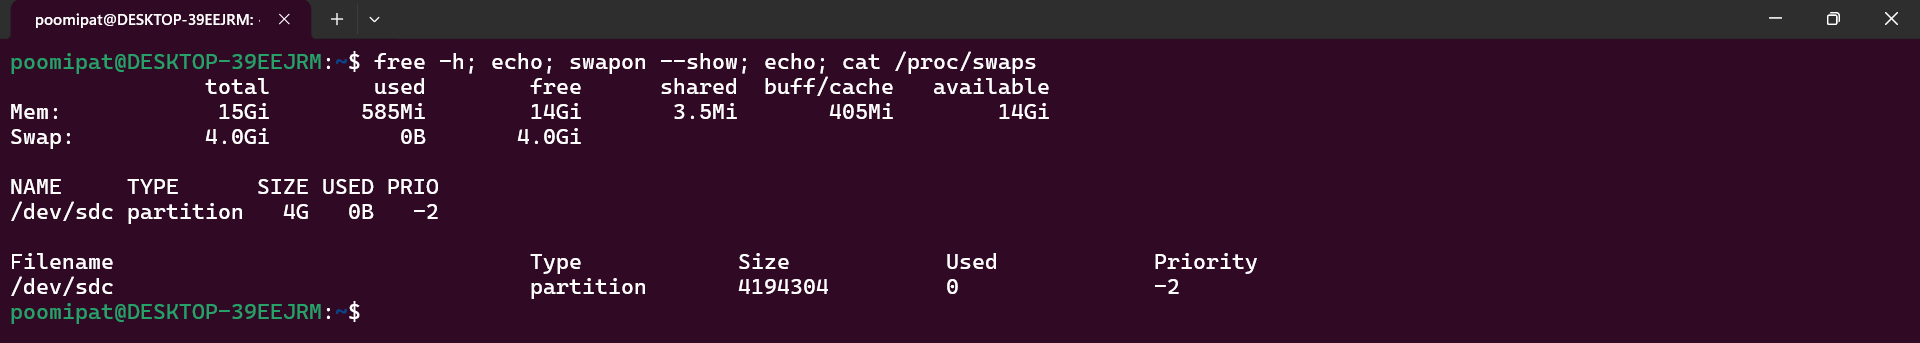
\includegraphics[width=\textwidth]{../result/screenshots/s01_swap_baseline.png}
\caption{สถานะตั้งต้น: swap เดิมมีเพียง partition \code{/dev/sdc} ขนาด 4 GiB}
\end{figure}

จากภาพ ระบบมีหน่วยความจำหลัก 15 GiB ใช้ไป 585 MiB และมี swap ทั้งหมด 4.0 GiB ที่ยังไม่ถูกใช้เลย (\code{used} เท่ากับ \code{0B}) โดย swap นี้เป็นชนิด partition ชื่อ \code{/dev/sdc} มีค่า priority เท่ากับ \code{-2} ส่วน \code{/proc/swaps} รายงานขนาดเป็นหน่วย KiB คือ 4194304 KiB ซึ่งเท่ากับ 4 GiB พอดี จุดที่ควรสังเกตคือ swap ก้อนนี้ไม่ได้เกิดจากการติดตั้ง Ubuntu เอง แต่เป็น virtual disk ที่ WSL2 สร้างให้อัตโนมัติ (ขนาดเริ่มต้นเท่ากับ 25\% ของ RAM ที่ virtual machine มองเห็น)

\subsubsection{ขั้นที่ 2: สร้าง file สำหรับใช้เป็น swap}

\begin{lstlisting}[style=terminal,caption={สร้าง file ขนาด 2 GiB ด้วย fallocate}]
sudo fallocate -l 2G /swapfile
ls -lh /swapfile
\end{lstlisting}

\begin{figure}[H]
\centering
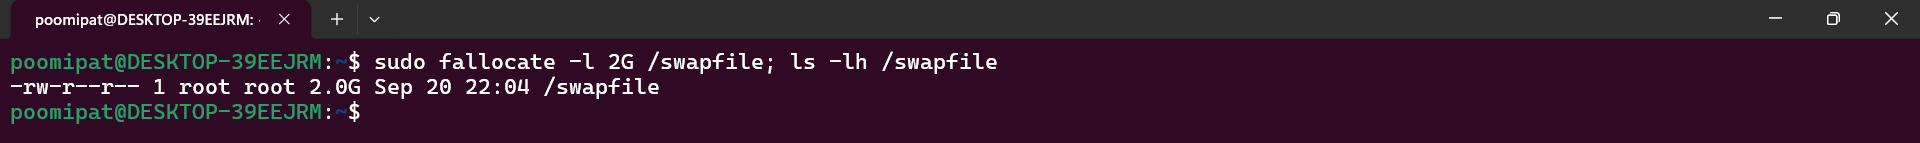
\includegraphics[width=\textwidth]{../result/screenshots/s02_fallocate.png}
\caption{\code{fallocate -l 2G} จองพื้นที่บน disk ให้ครบ 2 GiB ในคำสั่งเดียว}
\end{figure}

\code{fallocate} จองพื้นที่บน file system ให้ครบตามขนาดที่ระบุทันทีโดยไม่ต้องเขียนข้อมูลลงไปจริง จึงเร็วกว่าการใช้ \code{dd} มาก ผลที่ได้คือ file \code{/swapfile} ขนาด 2.0G เจ้าของเป็น \code{root} เพราะสร้างผ่าน \code{sudo} แต่สิทธิ์ที่ได้คือ \code{-rw-r--r--} (644) ซึ่งหมายความว่าผู้ใช้ทั่วไปอ่าน file นี้ได้ ถือเป็นช่องโหว่ร้ายแรงเพราะ swap เก็บข้อมูลที่ถูกย้ายออกจากหน่วยความจำของทุก process รวมถึงข้อมูลที่เป็นความลับ จึงต้องแก้สิทธิ์ในขั้นถัดไปก่อนนำไปใช้งาน

\textbf{ทางเลือก:} หาก file system ไม่รองรับ \code{fallocate} หรือ \code{swapon} ปฏิเสธ file ที่มีช่องว่าง (ข้อความ \code{it appears to have holes}) ให้สร้างด้วยการเขียนข้อมูลจริงแทน คือ \code{sudo dd if=/dev/zero of=/swapfile bs=1M count=2048}

\subsubsection{ขั้นที่ 3: ตั้งสิทธิ์และ format พื้นที่ให้เป็น swap area}

\begin{lstlisting}[style=terminal,caption={ปิดสิทธิ์ให้เหลือเฉพาะ root แล้วเขียน header ของ swap}]
sudo chmod 600 /swapfile
ls -lh /swapfile
sudo mkswap /swapfile
\end{lstlisting}

\begin{figure}[H]
\centering
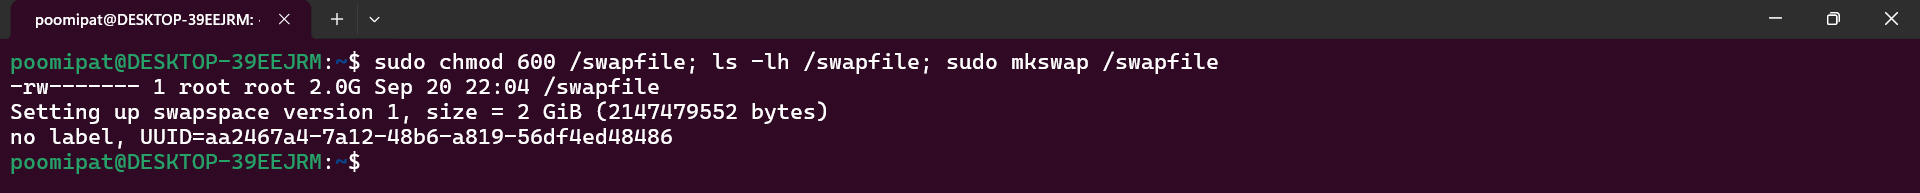
\includegraphics[width=\textwidth]{../result/screenshots/s03_mkswap.png}
\caption{หลัง \code{chmod 600} สิทธิ์เหลือเฉพาะ root และ \code{mkswap} เขียน header พร้อม UUID}
\end{figure}

สิทธิ์เปลี่ยนเป็น \code{-rw-------} คือมีเพียง \code{root} เท่านั้นที่อ่านหรือเขียนได้ จากนั้น \code{mkswap} จะเขียนโครงสร้าง header ของ swap area ลงไปที่ต้นของ file แล้วรายงานว่า \code{Setting up swapspace version 1, size = 2 GiB (2147479552 bytes)} พร้อมกำหนด UUID ให้หนึ่งค่า

ตัวเลขที่น่าสนใจคือ 2147479552 bytes ซึ่งน้อยกว่า 2 GiB (2147483648 bytes) อยู่ 4096 bytes พอดี ส่วนที่หายไปคือ page แรกของ file ที่ถูกกันไว้เก็บ header ของ swap area จึงเหลือพื้นที่ใช้งานจริง 2097148 KiB ตามที่จะเห็นใน \code{/proc/swaps} ในขั้นถัดไป

\subsubsection{ขั้นที่ 4: เปิดใช้งาน swap file}

\begin{figure}[H]
\centering
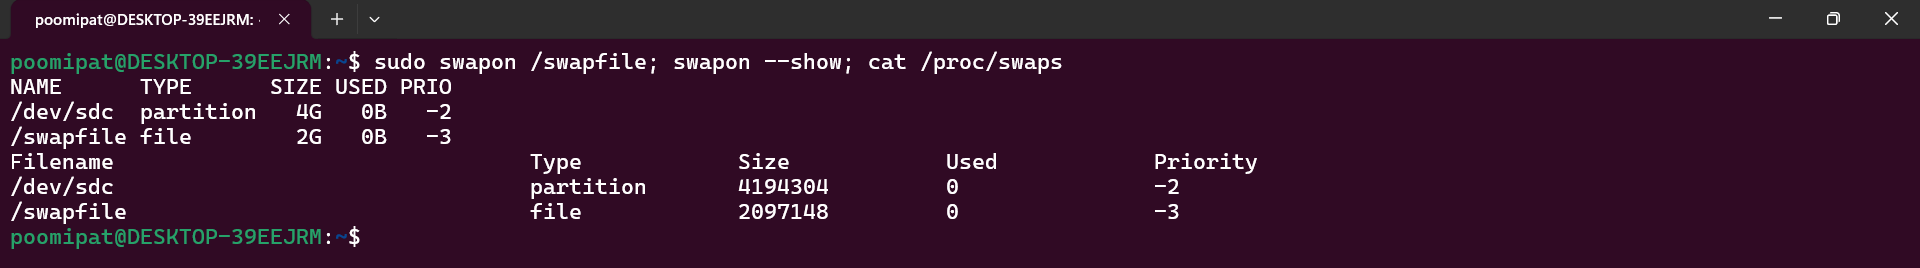
\includegraphics[width=\textwidth]{../result/screenshots/s04_swapon.png}
\caption{หลัง \code{swapon} ระบบมี swap area สองก้อนทำงานพร้อมกัน}
\end{figure}

หลังสั่ง \code{sudo swapon /swapfile} ระบบมี swap area สองก้อนคือ partition \code{/dev/sdc} ขนาด 4G และ file \code{/swapfile} ขนาด 2G ทั้งสองก้อนยังมี \code{USED} เป็น \code{0B} เพราะหน่วยความจำยังเหลือเฟือ

ค่า \code{PRIO} เป็นจุดที่ควรอธิบายเพิ่ม เมื่อไม่ได้ระบุ priority เอง kernel จะไล่ค่าติดลบลงเรื่อย ๆ ตามลำดับการเปิดใช้งาน swap ก้อนแรกจึงได้ \code{-2} และก้อนที่เปิดทีหลังได้ \code{-3} kernel จะใช้ swap ที่มี priority สูงกว่าก่อนเสมอ ในที่นี้คือใช้ partition จนเต็มแล้วจึงลงมาใช้ swap file หากต้องการให้ใช้พร้อมกันแบบกระจายโหลด ต้องกำหนด priority ให้เท่ากันด้วย \code{swapon -p} หรือใส่ option \code{pri=} ใน \code{/etc/fstab}

\subsubsection{ขั้นที่ 5: ยืนยันว่า swap เพิ่มขึ้นจริง}

\begin{figure}[H]
\centering
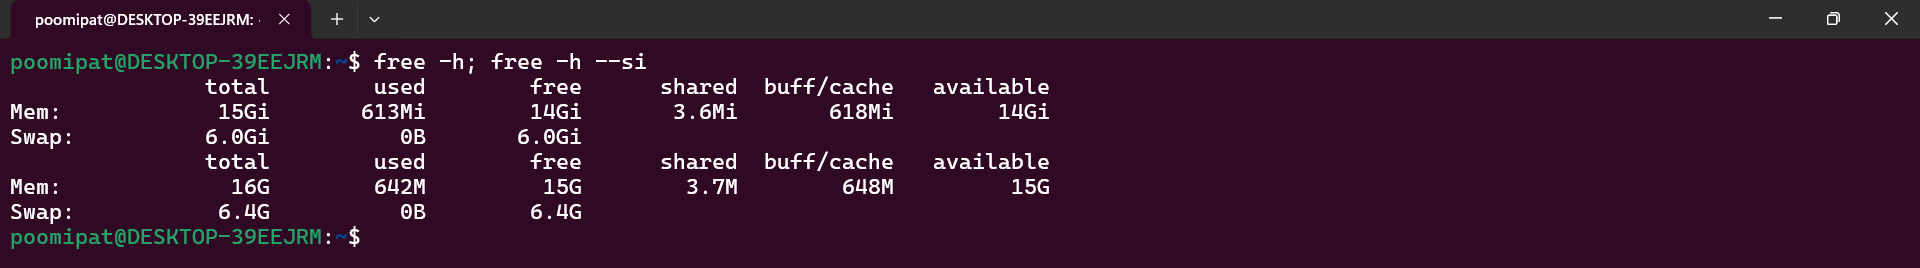
\includegraphics[width=\textwidth]{../result/screenshots/s05_free_after_add.png}
\caption{\code{Swap} total เพิ่มจาก 4.0Gi เป็น 6.0Gi และการเทียบหน่วยฐาน 1024 กับฐาน 1000}
\end{figure}

บรรทัด \code{Swap} แสดง total เท่ากับ 6.0Gi ซึ่งคือ 4 GiB ของ partition เดิมบวกกับ 2 GiB ของ swap file ที่เพิ่งเพิ่มเข้าไป เท่ากับว่าการเพิ่ม swap สำเร็จตามเป้าหมาย

คำสั่งที่สองในภาพคือ \code{free -h --si} ซึ่งให้ผลเป็น 6.4G และ 16G เพราะ \code{--si} เปลี่ยนไปใช้หน่วยฐาน 1000 (GB) แทนฐาน 1024 (GiB) ตัวเลขที่ต่างกันนี้ไม่ได้แปลว่าหน่วยความจำเปลี่ยน เป็นเพียงการเลือกฐานของหน่วยที่ต่างกันเท่านั้น

\subsubsection{ขั้นที่ 6: ทำให้ถาวร และข้อจำกัดที่พบบน WSL2}

บน Linux ทั่วไป การทำให้ swap file กลับมาเองหลัง reboot ทำได้ด้วยการเพิ่มบรรทัดต่อไปนี้ลงใน \code{/etc/fstab}

\begin{lstlisting}[style=terminal,caption={รูปแบบของบรรทัด swap ใน /etc/fstab}]
/swapfile none swap sw 0 0
\end{lstlisting}

ทั้งหกช่องมีความหมายตามลำดับคือ อุปกรณ์หรือ file ที่จะใช้, จุด mount (swap ไม่มีจุด mount จึงใส่ \code{none}), ชนิดของ file system (\code{swap}), option (\code{sw} คือค่าเริ่มต้นสำหรับ swap), ค่าสำหรับ \code{dump} และลำดับการตรวจ file system ด้วย \code{fsck} ซึ่ง swap ไม่ต้องตรวจจึงเป็น \code{0} ทั้งสองช่อง

\begin{figure}[H]
\centering
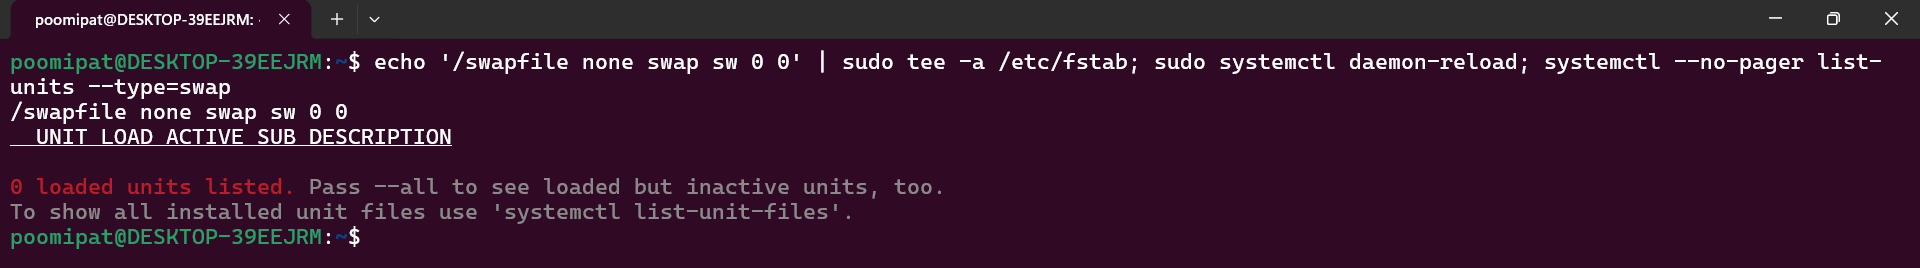
\includegraphics[width=\textwidth]{../result/screenshots/s06_fstab.png}
\caption{บรรทัดเข้า \code{/etc/fstab} สำเร็จ แต่ systemd ตอบว่าไม่มี swap unit ที่ load อยู่เลย}
\end{figure}

ผลที่ได้กลับไม่เป็นไปตามตำราคือ หลังสั่ง \code{systemctl daemon-reload} แล้วตรวจด้วย \code{systemctl list-units --type=swap} ระบบตอบว่า \code{0 loaded units listed} แสดงว่า systemd ไม่ได้สร้าง unit ชื่อ \code{swapfile.swap} ให้ตามที่ควรจะเป็น เมื่อไล่หาสาเหตุจาก journal ของระบบพบข้อความที่ชี้สาเหตุโดยตรง

\begin{figure}[H]
\centering
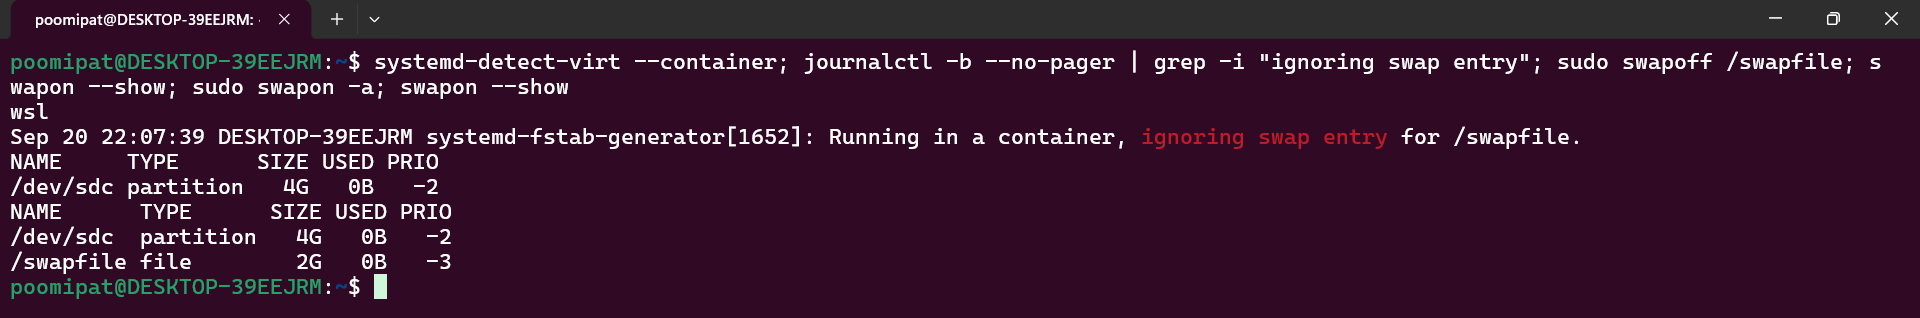
\includegraphics[width=\textwidth]{../result/screenshots/s06b_container_ignored.png}
\caption{สาเหตุที่แท้จริง: systemd มองว่า WSL2 เป็น container จึงข้าม swap entry ใน \code{/etc/fstab}}
\end{figure}

ภาพนี้อธิบายเรื่องทั้งหมดได้ในภาพเดียว เริ่มจาก \code{systemd-detect-virt --container} ตอบว่า \code{wsl} คือ systemd รู้ตัวว่ากำลังทำงานอยู่ภายใน container จากนั้นบรรทัดที่ดึงมาจาก journal ระบุชัดว่า \code{systemd-fstab-generator: Running in a container, ignoring swap entry for /swapfile.} กล่าวคือ ตัว generator ที่ทำหน้าที่แปลง \code{/etc/fstab} เป็น systemd unit จะ \textbf{ข้ามบรรทัด swap ทุกบรรทัดทิ้งเมื่อทำงานอยู่ใน container} เพราะตามหลักการแล้ว container ไม่ควรจัดการ swap ของเครื่องเอง

เพื่อพิสูจน์ว่าบรรทัดใน \code{/etc/fstab} นั้นถูกต้อง ภาพเดียวกันจึงทดสอบต่อด้วยการสั่ง \code{swapoff} ให้เหลือ swap ก้อนเดียวก่อน แล้วสั่ง \code{sudo swapon -a} ซึ่งเป็นคำสั่งที่อ่าน \code{/etc/fstab} โดยตรงไม่ผ่าน systemd ผลคือ \code{/swapfile} กลับมาทำงานอีกครั้งพร้อม priority \code{-3} เหมือนเดิม สรุปได้ว่าปัญหาไม่ได้อยู่ที่บรรทัดใน \code{/etc/fstab} แต่อยู่ที่ systemd บน WSL2 ต่างหากที่เลือกจะไม่อ่านมัน

\textbf{วิธีทำให้ swap ถาวรบน WSL2} มีสองทางที่ใช้ได้จริง

\begin{enumerate}[leftmargin=*]
  \item สั่ง \code{swapon -a} ตอน WSL2 เริ่มทำงาน โดยเพิ่มค่าต่อไปนี้ใน \code{/etc/wsl.conf} ฝั่ง Linux
  \begin{lstlisting}[style=terminal]
[boot]
command = swapon -a
  \end{lstlisting}
  \item ปรับขนาด swap ที่ WSL2 สร้างให้เองแทนการเพิ่ม swap file ใหม่ โดยสร้าง file \code{C:\textbackslash Users\textbackslash <user>\textbackslash .wslconfig} ฝั่ง Windows แล้วกำหนด
  \begin{lstlisting}[style=terminal]
[wsl2]
swap = 8GB
  \end{lstlisting}
  จากนั้นสั่ง \code{wsl --shutdown} ให้ virtual machine ปิดแล้วเปิดใหม่ ขนาดของ partition \code{/dev/sdc} จะเปลี่ยนตามค่าที่ตั้งไว้ วิธีนี้เป็นวิธีที่ตรงกับสถาปัตยกรรมของ WSL2 มากที่สุด เพราะ swap ของ WSL2 ถูกจัดการจากฝั่ง Windows ไม่ใช่จากฝั่ง Linux
\end{enumerate}

\subsubsection{ขั้นที่ 7: ลด swap space}

\begin{figure}[H]
\centering
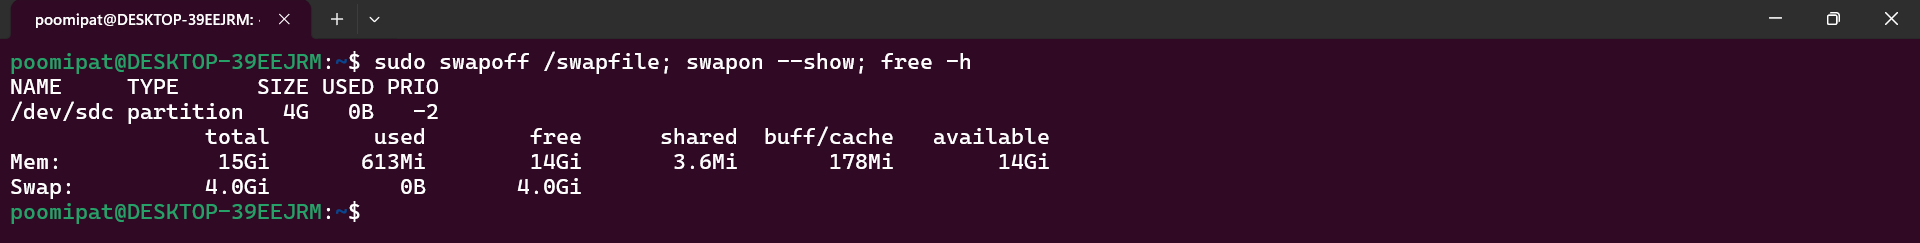
\includegraphics[width=\textwidth]{../result/screenshots/s07_swapoff.png}
\caption{\code{swapoff} ปิดการใช้งาน swap file ทำให้ swap รวมลดจาก 6.0Gi กลับเป็น 4.0Gi}
\end{figure}

การลด swap ทำได้ด้วยคำสั่ง \code{sudo swapoff /swapfile} ซึ่งจะย้าย page ทั้งหมดที่ค้างอยู่ใน swap area ก้อนนั้นกลับเข้าหน่วยความจำหลักหรือย้ายไป swap ก้อนอื่นก่อน แล้วจึงถอด swap area ออกจากระบบ ข้อควรระวังคือ \textbf{ต้องมีหน่วยความจำว่างพอจะรับ page เหล่านั้นกลับ} มิฉะนั้นคำสั่งจะล้มเหลวด้วยข้อความ \code{Cannot allocate memory} ในการทดลองนี้ swap ยังไม่ถูกใช้งานเลย คำสั่งจึงจบทันที ผลลัพธ์คือเหลือ swap เพียง \code{/dev/sdc} และ \code{Swap} total กลับเป็น 4.0Gi

อีกจุดที่สังเกตได้คือ \code{buff/cache} ลดจาก 618 MiB เหลือ 178 MiB เพราะ page cache ที่ระบบใช้กับ file \code{/swapfile} ถูกปล่อยคืนไปพร้อมกัน

\subsubsection{ขั้นที่ 8: ลบ file และคืนค่าระบบให้เหมือนเดิม}

\begin{figure}[H]
\centering
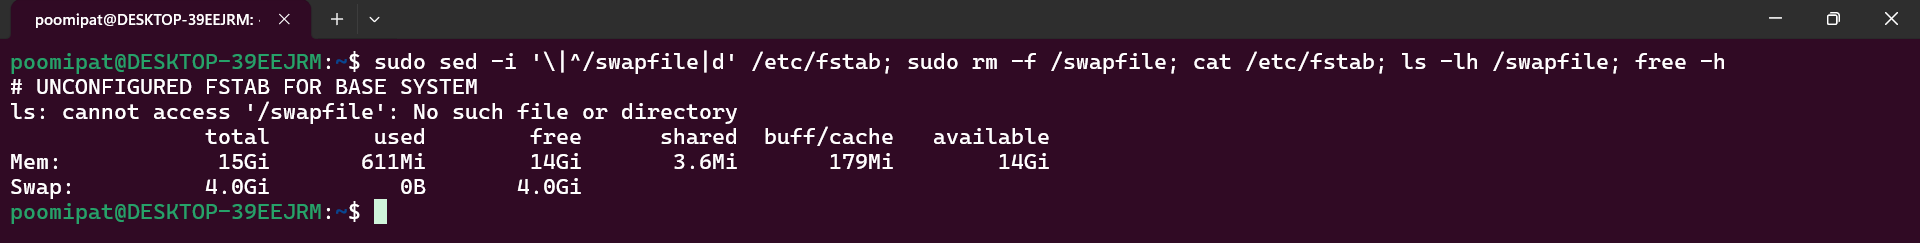
\includegraphics[width=\textwidth]{../result/screenshots/s08_cleanup.png}
\caption{ลบบรรทัดใน \code{/etc/fstab} และลบ file ทิ้ง ระบบกลับสู่สภาพก่อนการทดลอง}
\end{figure}

เมื่อ swap file ถูกปิดการใช้งานแล้วจึงลบ file ทิ้งได้อย่างปลอดภัยด้วย \code{sudo rm /swapfile} พร้อมกับลบบรรทัดที่เพิ่มไว้ใน \code{/etc/fstab} ออก ภาพแสดงว่า \code{/etc/fstab} เหลือเพียงบรรทัดคอมเมนต์เดิม และ \code{ls} รายงาน \code{No such file or directory} ซึ่งยืนยันว่า file ถูกลบจริง ส่วน \code{Swap} total คือ 4.0Gi เท่ากับตอนเริ่มต้นการทดลองทุกประการ

\textbf{ลำดับที่ห้ามสลับ:} ต้องสั่ง \code{swapoff} ก่อนลบ file เสมอ หากลบ file ทิ้งขณะที่ swap ยังเปิดใช้งานอยู่ kernel จะยังอ้างถึงพื้นที่นั้นต่อไปจนกว่าจะ reboot และอาจทำให้ระบบไม่เสถียร

\subsubsection{การปรับพฤติกรรมการใช้ swap ด้วย vm.swappiness}

การเพิ่มหรือลดขนาด swap เป็นการเปลี่ยน \textit{ปริมาณ} ที่มีให้ใช้ ส่วนการปรับ \code{vm.swappiness} เป็นการเปลี่ยน \textit{ความเต็มใจ} ของ kernel ที่จะใช้ swap ซึ่งมักต้องทำควบคู่กัน

\begin{figure}[H]
\centering
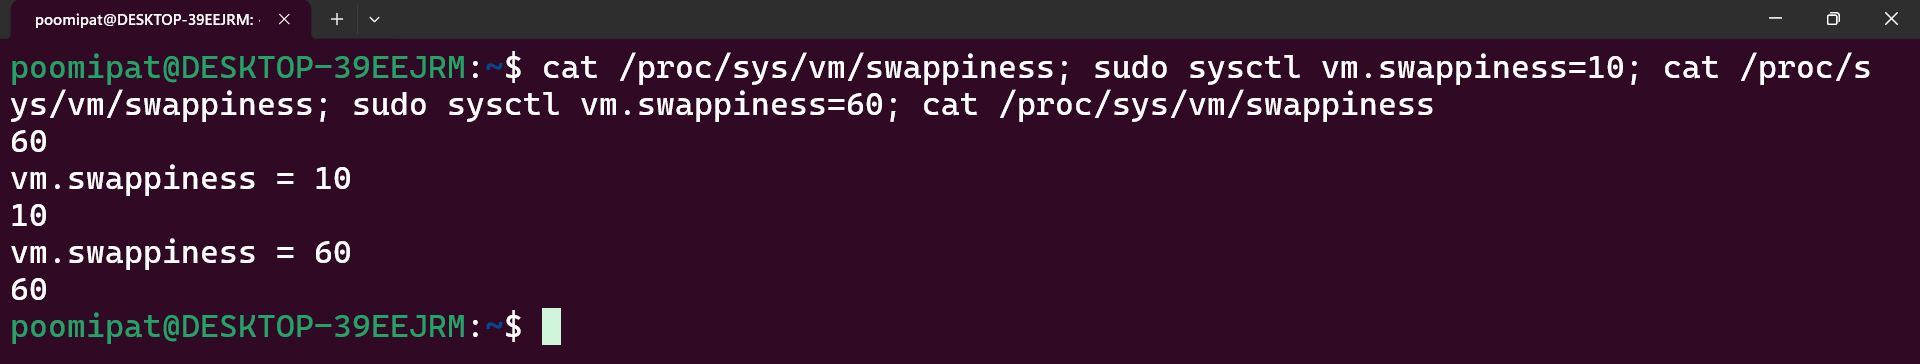
\includegraphics[width=\textwidth]{../result/screenshots/s09_swappiness.png}
\caption{ปรับ \code{vm.swappiness} จาก 60 เป็น 10 แล้วตั้งกลับเป็น 60}
\end{figure}

ค่าเริ่มต้นของระบบคือ 60 เมื่อสั่ง \code{sudo sysctl vm.swappiness=10} ค่าใน \code{/proc/sys/vm/swappiness} เปลี่ยนเป็น 10 ทันทีโดยไม่ต้อง reboot ค่าที่ต่ำลงหมายความว่า kernel จะพยายามเรียกคืน page cache ก่อนและหลีกเลี่ยงการย้าย anonymous page ลง swap ส่วนค่าที่สูงขึ้นหมายถึงยอมใช้ swap ได้ง่ายขึ้น การทดลองจบลงด้วยการตั้งค่ากลับเป็น 60 เพื่อคืนสภาพระบบ

ค่าที่ตั้งด้วย \code{sysctl} จะหายไปเมื่อ reboot หากต้องการให้ถาวรต้องเพิ่มบรรทัด \code{vm.swappiness=10} ลงใน \code{/etc/sysctl.conf} หรือสร้าง file ใหม่ใน \code{/etc/sysctl.d/}

\subsubsection{สรุปคำสั่งทั้งหมดของข้อ 1.2}

\begin{table}[H]
\centering\small
\caption{สรุปคำสั่งสำหรับเพิ่มและลด swap space บน Linux}
\begin{tabular}{@{}p{2.2cm}p{6.6cm}p{6.8cm}@{}}
\toprule
\textbf{เป้าหมาย} & \textbf{คำสั่ง} & \textbf{หน้าที่} \\
\midrule
เพิ่ม swap & \code{sudo fallocate -l 2G /swapfile} & จองพื้นที่บน disk ขนาด 2 GiB \\
 & \code{sudo chmod 600 /swapfile} & ปิดสิทธิ์ให้เหลือเฉพาะ root \\
 & \code{sudo mkswap /swapfile} & เขียน header ของ swap area และกำหนด UUID \\
 & \code{sudo swapon /swapfile} & สั่งให้ kernel เริ่มใช้งาน swap area นี้ \\
 & \code{echo ... | sudo tee -a /etc/fstab} & ทำให้กลับมาเองหลัง reboot (ดูข้อจำกัดบน WSL2) \\
\midrule
ลด swap & \code{sudo swapoff /swapfile} & ย้าย page กลับเข้า RAM แล้วถอด swap area ออก \\
 & \code{sudo rm /swapfile} & ลบ file ทิ้งหลังปิดการใช้งานแล้วเท่านั้น \\
 & แก้ \code{/etc/fstab} & ลบบรรทัดที่เพิ่มไว้ออก \\
\midrule
ตรวจสอบ & \code{free -h}, \code{swapon --show}, \code{cat /proc/swaps} & ดูขนาดและสถานะการใช้งานของ swap \\
\midrule
ปรับพฤติกรรม & \code{sudo sysctl vm.swappiness=10} & เปลี่ยนแนวโน้มที่ kernel จะใช้ swap \\
\bottomrule
\end{tabular}
\end{table}
